\section{Exploratory Data Analysis}

One effective way to understand and explore a dataset is through visualization of the feature distribution for each class.
However, when the number of features is high, such as 728 in this case, this method may not be practical or informative.
In these situations, alternative approaches for visualizing the dataset can be utilized to extract useful insights.

\subsection{Principal Component Analysis}
One way to gain insights from a large dataset that may be difficult to visualize is through the use of principal component analysis (PCA).
PCA is a technique that reduces the number of features in a dataset while preserving the most important information.
It does this by transforming the original variables into a new set of variables called principal components, which are uncorrelated and capture the maximum amount of variance in the data.
In the following analysis, we will investigate the relationships between the first three principal components.

\begin{figure}[H]
    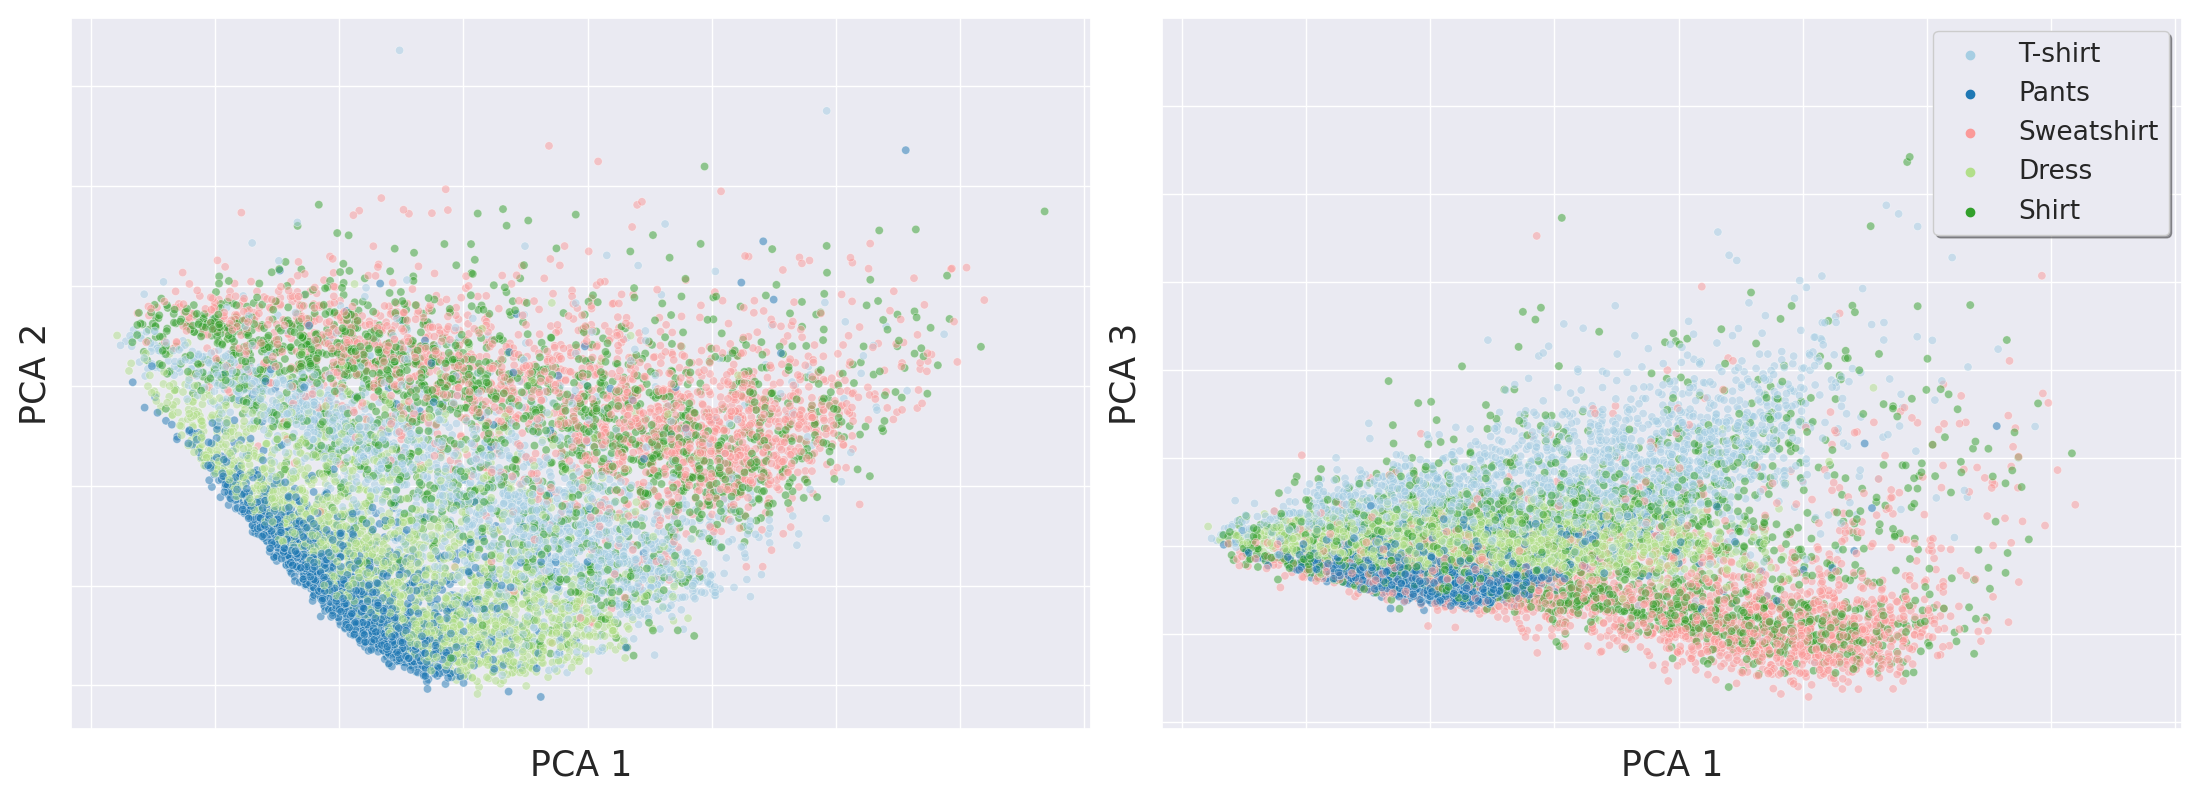
\includegraphics[scale=0.30]{figures_for_report/PCA}
    \captionsetup{justification=centering,margin=2cm}
    \caption{Visualizing relationships between the first 3 principal components}
\end{figure}

The first 3 principal components explain $42.7\%$ variance, and it requires 61 principal components to explain above $90\%$ variance.
The pca plots are a useful tool to visualize how well the classes are seperated and gives a general idea of which classes might be easier and harder to classify correctly.
Figure 3 shows that there is a clear overlap between many of the classes, especially between shirts and pullovers, which can potentially give a classifier trouble distinguishing between these two.

